\documentclass[a4paper,12pt]{scrartcl}

\usepackage[T1]{fontenc}
\usepackage{amsmath}
\usepackage{graphicx}
\usepackage{float}
\usepackage{xcolor}
\usepackage{authblk} % Allows for authors from multiiple institutes

\title{
\includegraphics[width=10cm]{DESYTestBeam.png}  
\includegraphics[width=10cm]{Aida2020.png} \\ \vspace{2cm} USER MANUAL \\ Slow Control System}
\author[*]{Lars Fischer}
%\author[*]{Mengqing Wu}
\affil[*]{Deutsches Elektronen-Synchrotron DESY, Notkestr. 85, 22607 Hamburg, Germany}

\date{January 2018}

\begin{document}
\maketitle
This document serves as a how-to manual for the Slow Control System that is easy to follow. Hardware and software will be introduced. The DAQ software consists of a commercial DAQ, called AMR and the EUDAQ. A detailed instruction to configure and use the DAQ system to get a measurement using all the connected sensors will be given.
\pagebreak

\tableofcontents
\pagebreak

\section{Introduction}
The Slow Control System collects data which can be included into other experimental data streams. To read more about a detailed description of use and installation of the structure see the deliverable report or the Main User Manual. \\
Deliverable Report: https://cds.cern.ch/record/2290758/files/AIDA-2020-D15\_3.3.pdf \\
Main User Manual: https://cds.cern.ch/record/2284369/files/AIDA-2020-NOTE-2017-007.pdf \\
This document will guide you step by step through all necessary installations and commands.

\section{Testbeam Facilities}
\begin{figure} [H]
\centering
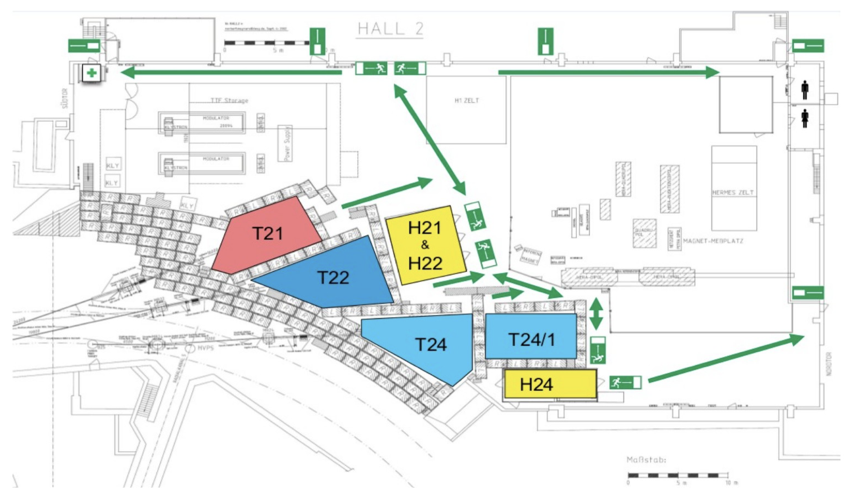
\includegraphics[width=\textwidth]{Testbeam.png}
\caption{Slow Control System Racks can be moved in T21/T22/T24 for observing.}
\end{figure}

The test beam facilities at DESY include three experimental areas in which the Slow Control System can be moved for monitoring. Each rack provides a set of \textbf{10 NTC sensors} with each 10 meters of cable so they can be placed as needed in the areas. These NTC sensors should be used in the temperature range of -20$^\circ$C to +100$^\circ$C. In addition \textbf{one DIGI sensor} is mounted fixed to the Slow Control rack and should not be moved. It collects temperature, humidity, air pressure and dew point data and transfers them to the ALMEMO data logger built by Ahlborn company. The data logger is connected to a Windows-PC mounted to the rack. The user is also able to attach their own sensors to the data collector. Therefore spare connectores are available in the rack.
An extra pair of LEDs on the top of the Slow Control System might be used for user defined warning signals. The power and Internet connection should always be interconnected while the Slow Control System is in use. The user is able to roll the data collection rack among different test beam areas or even to other work space. \\

\begin{figure} [H]
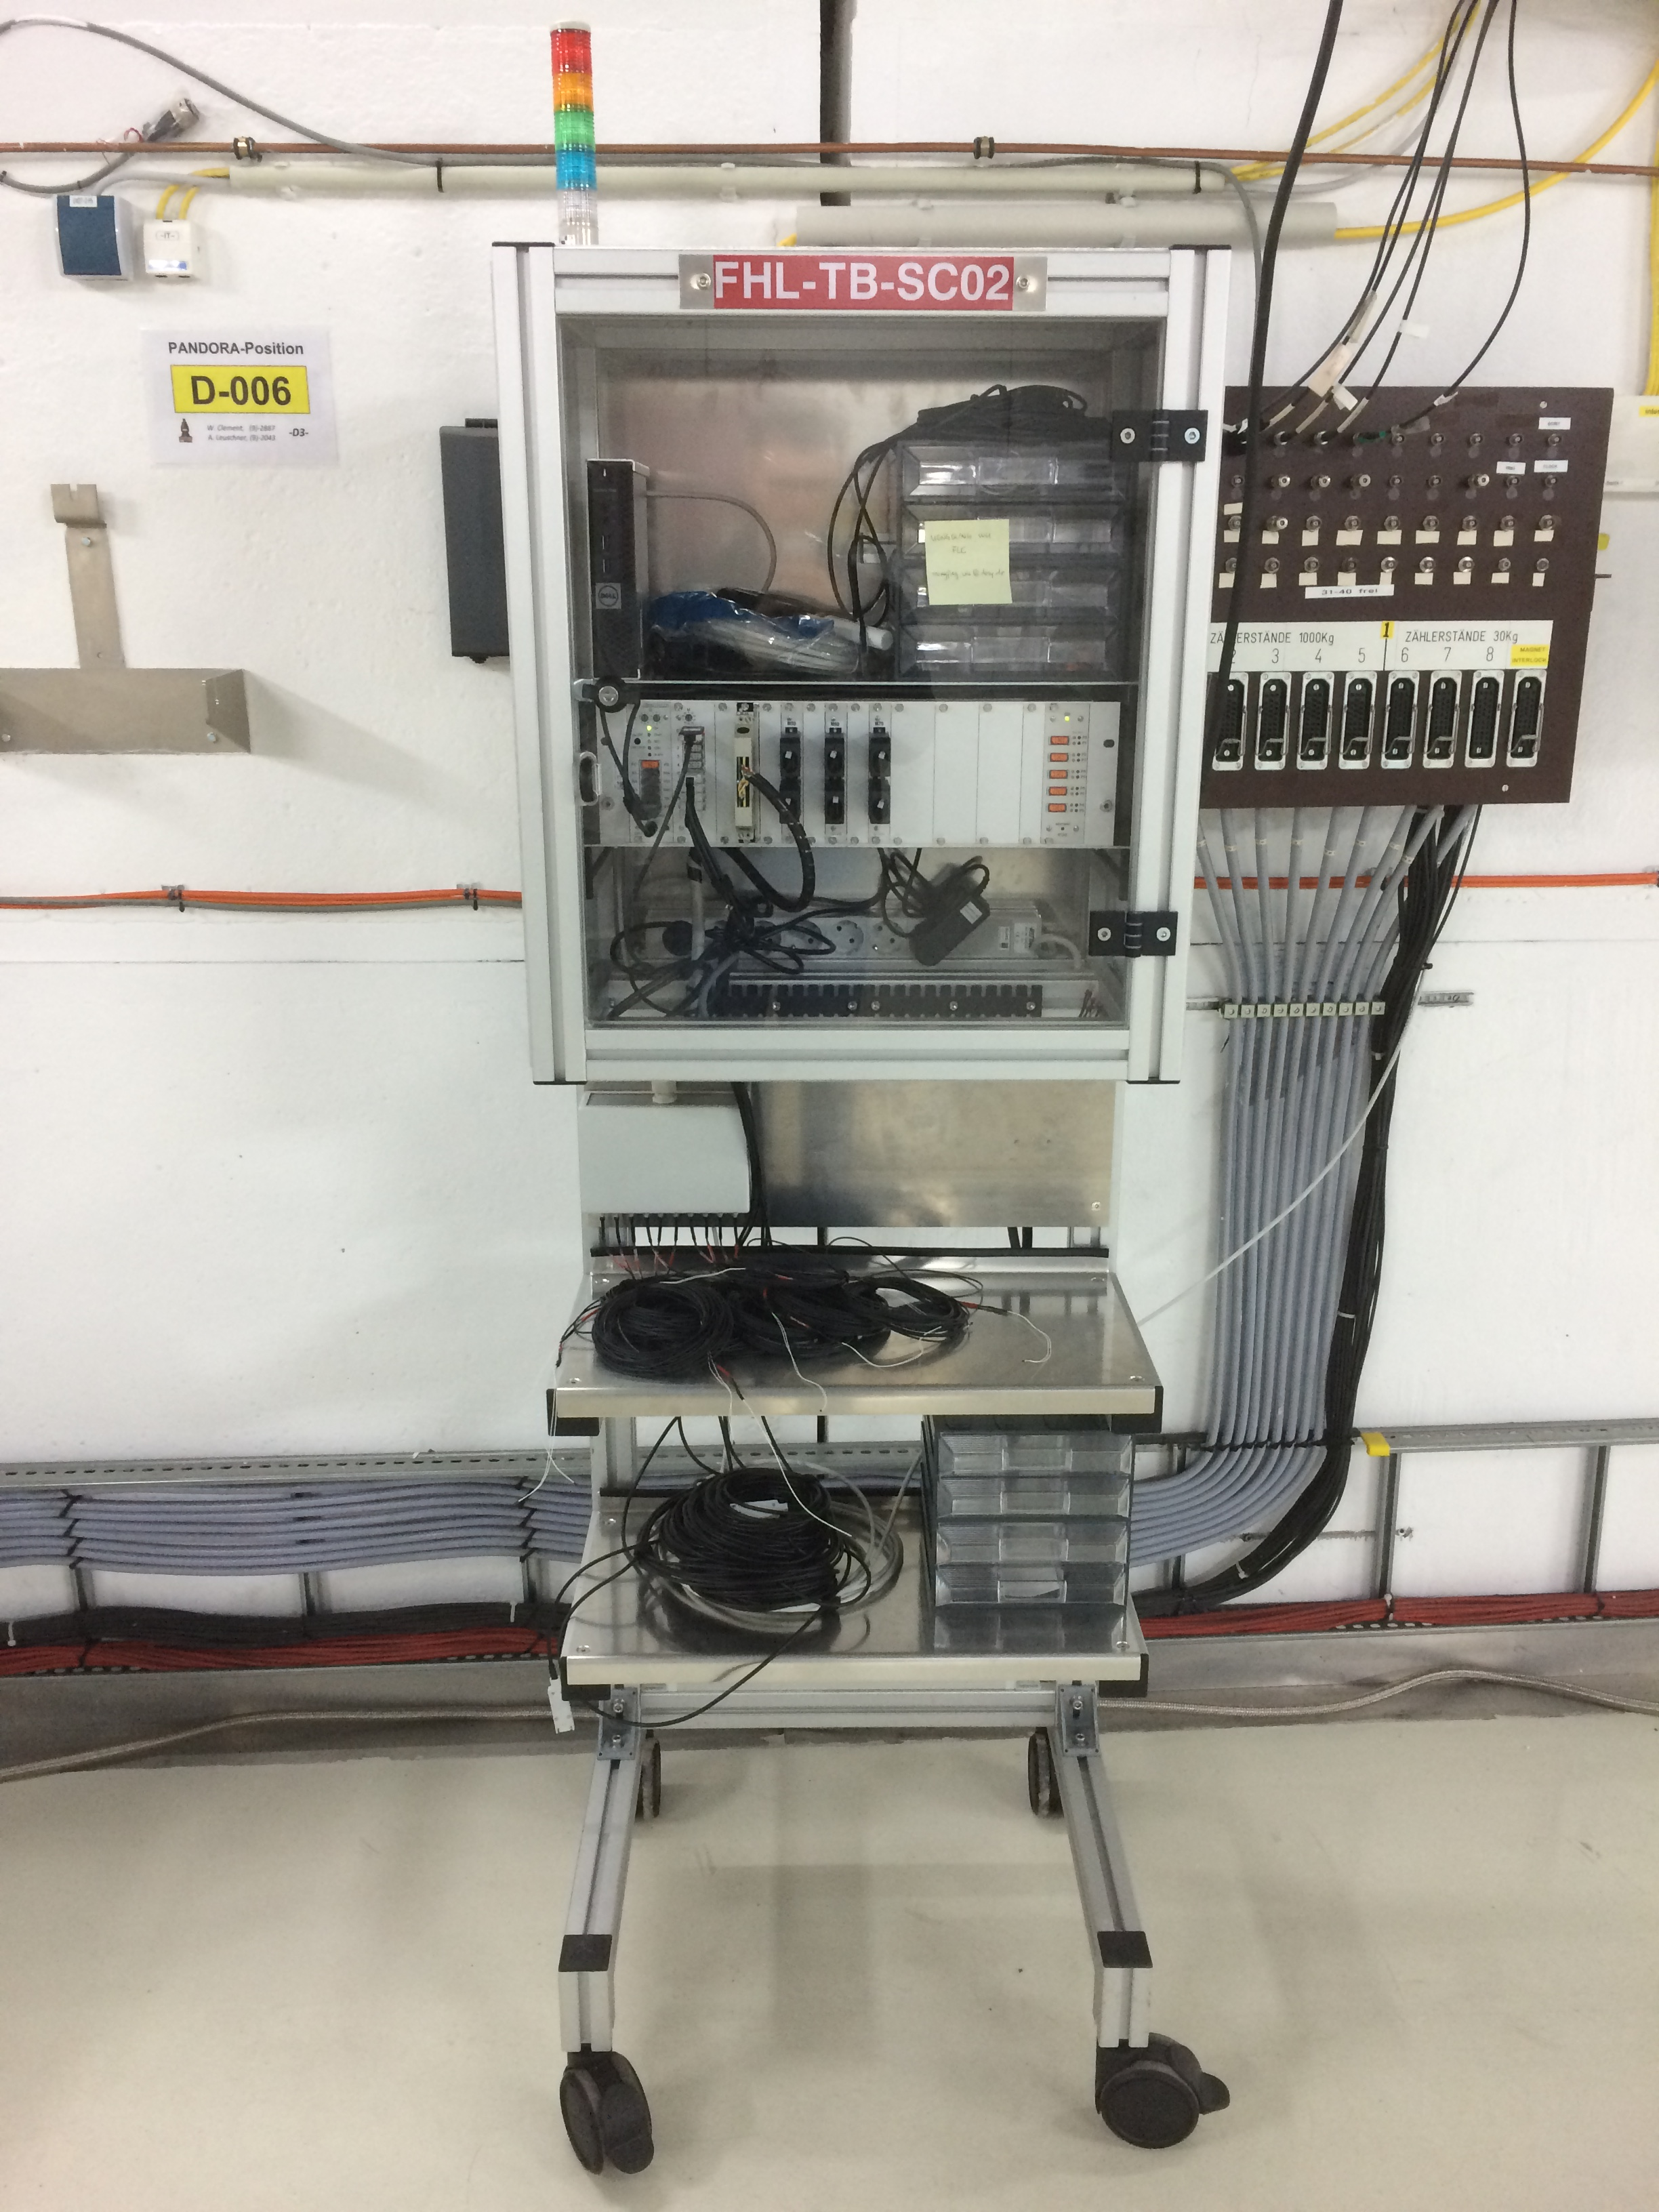
\includegraphics[width=5.6cm]{Rackganz.jpg} 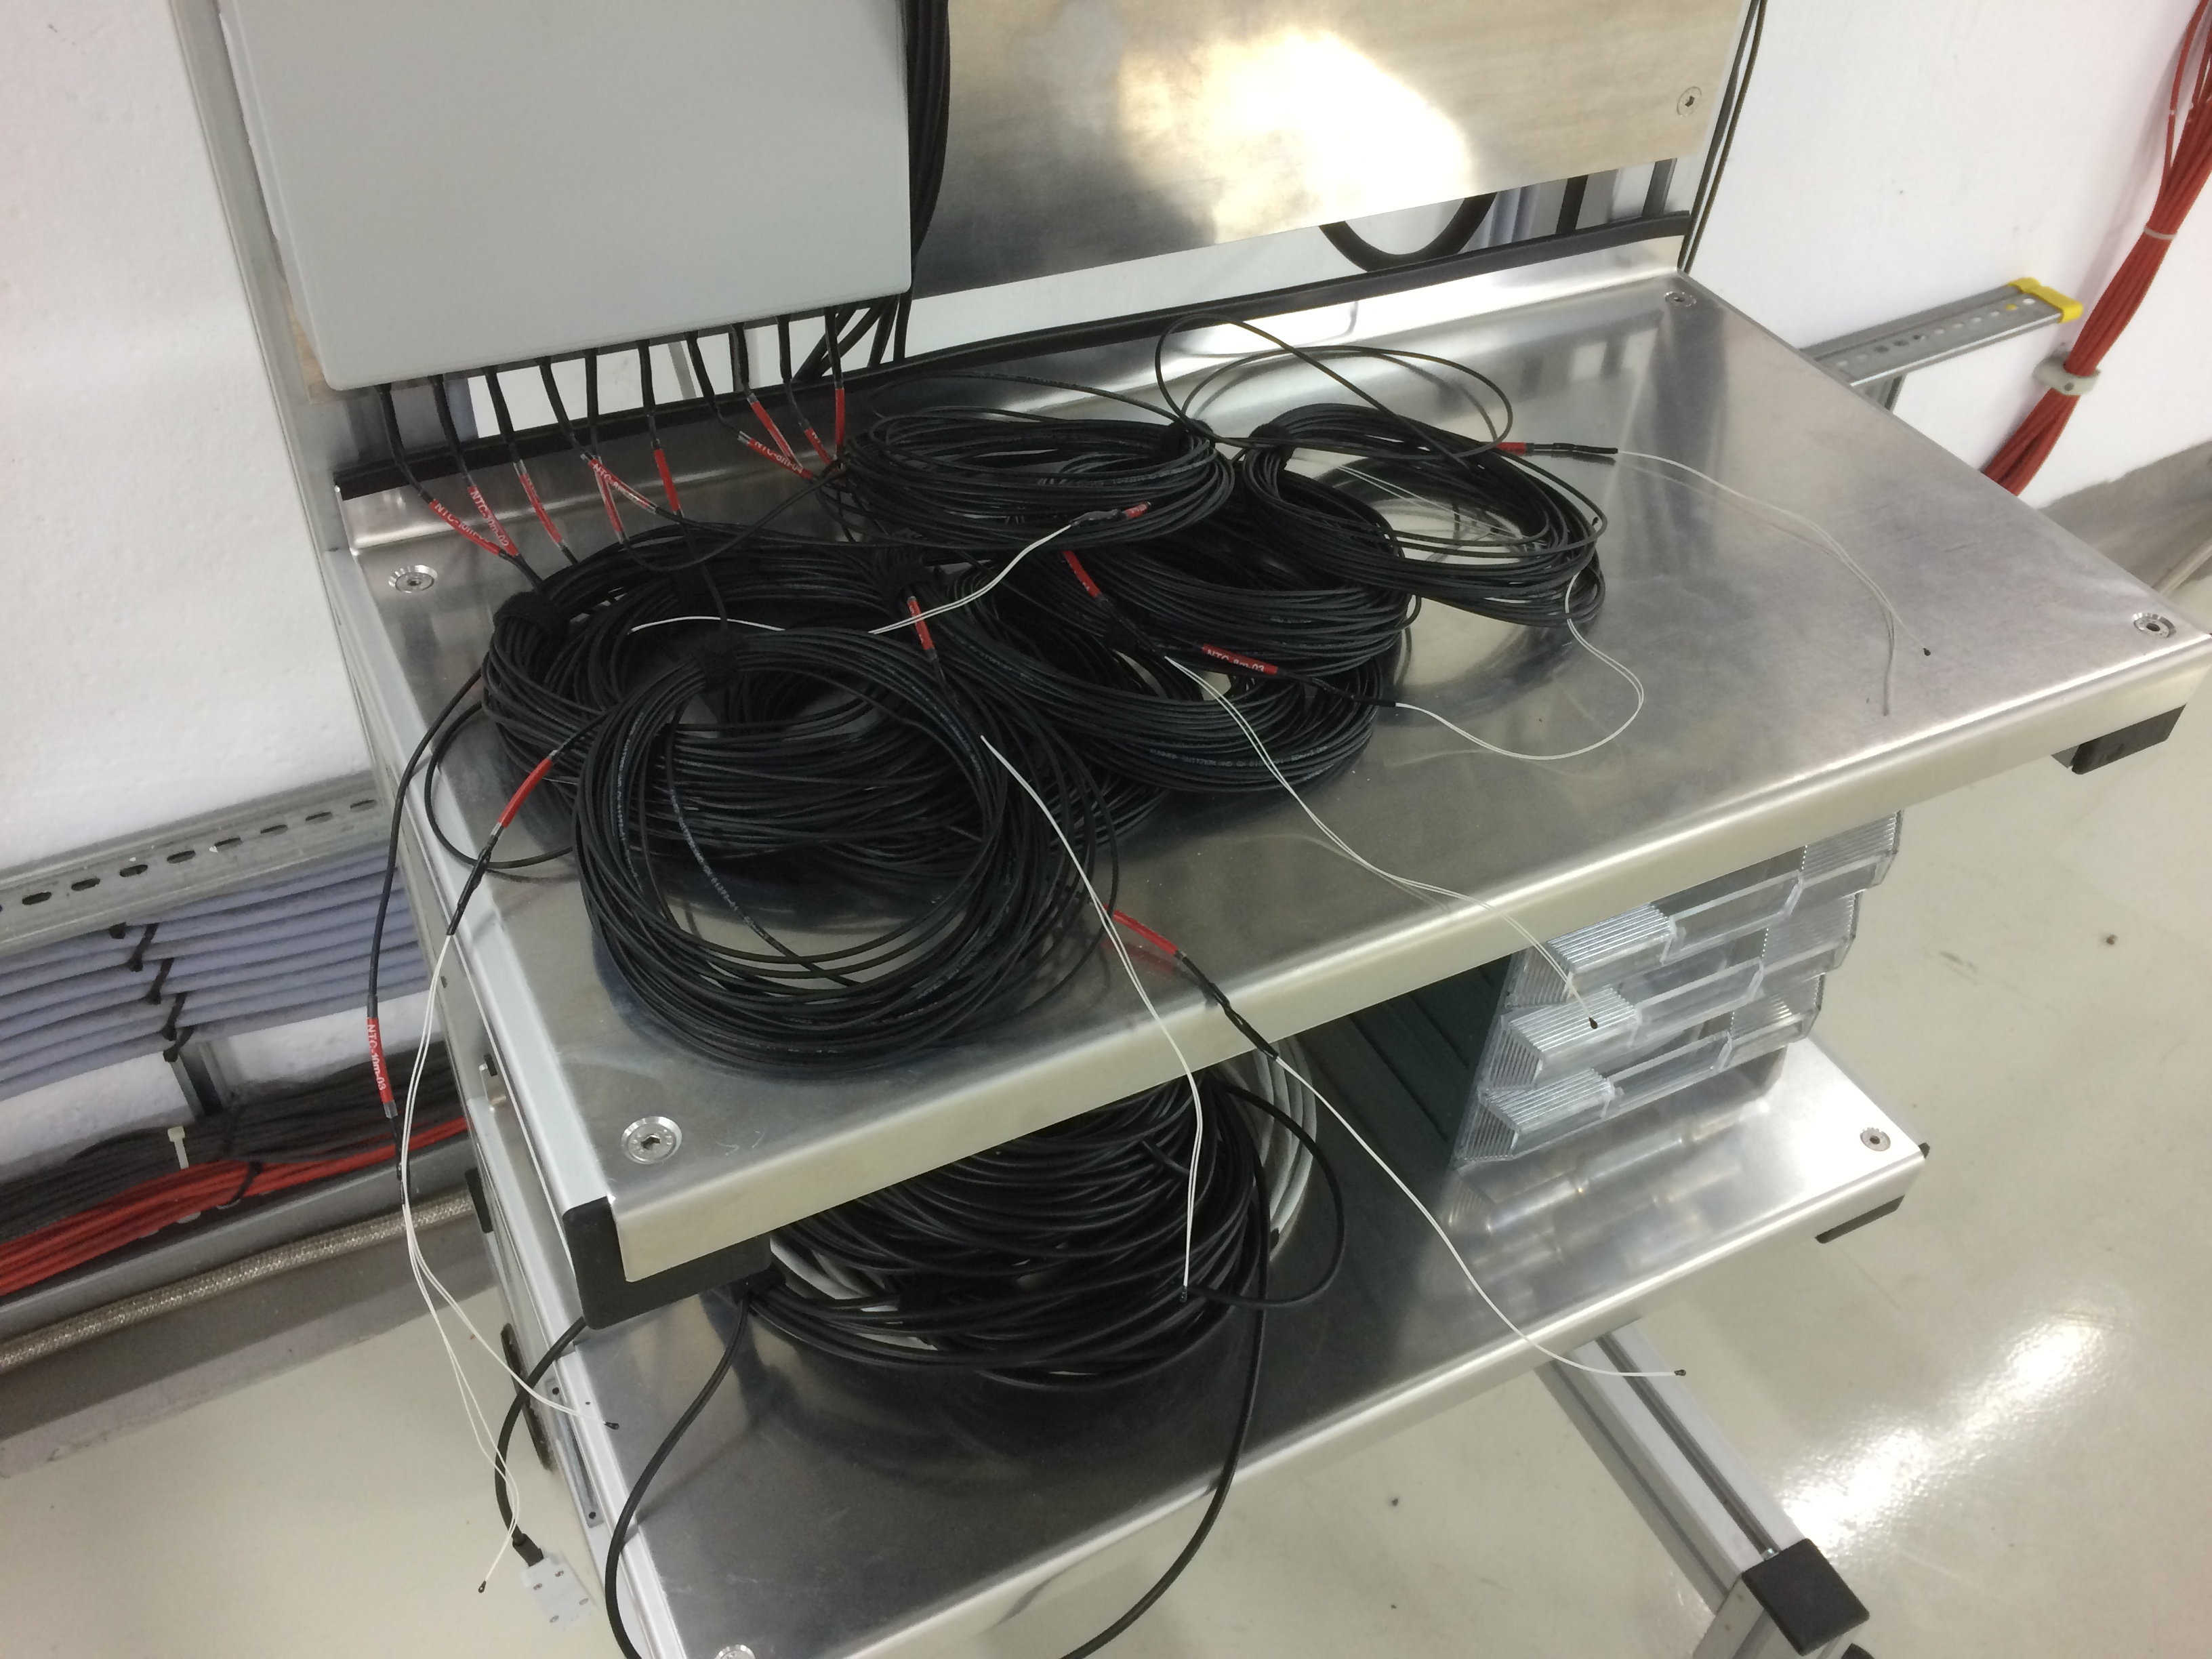
\includegraphics[width=10cm]{Sensoren.jpg}
\caption{Slow Control System rack 02 (left) in test beam area 24
and the 10  NTC sensors (right)}
\end{figure}

\section{Software Setup}
For data acquisition two PCs run in parallel (Figure 3). On the one hand the Windows PC on the rack collects the data from data logger (ALMEMO) with a commercial DAQ software (AMR). With the current adjustments the data logger transfers data from the sensors every 30 seconds to the AMR software. An ODBC is set up to forward the values into a MySQL (version 5.7.20) based database on the Linux-PC. On the other hand the EUDAQ software collects data in user defined timestamps from the database on the Linux PC. A unix-ODBC connection is the interface between the database and EUDAQ framework.
While the data is transfered into the database the second DAQ software collects only the events of the timestamps the user adjusted. The EUDAQ can simply be handled by an own GUI.
After data taking the output has to be converted from EUDAQ native formate into a csv file. There are macros provided for plotting the csv data in different variations.

\begin{figure} [H]
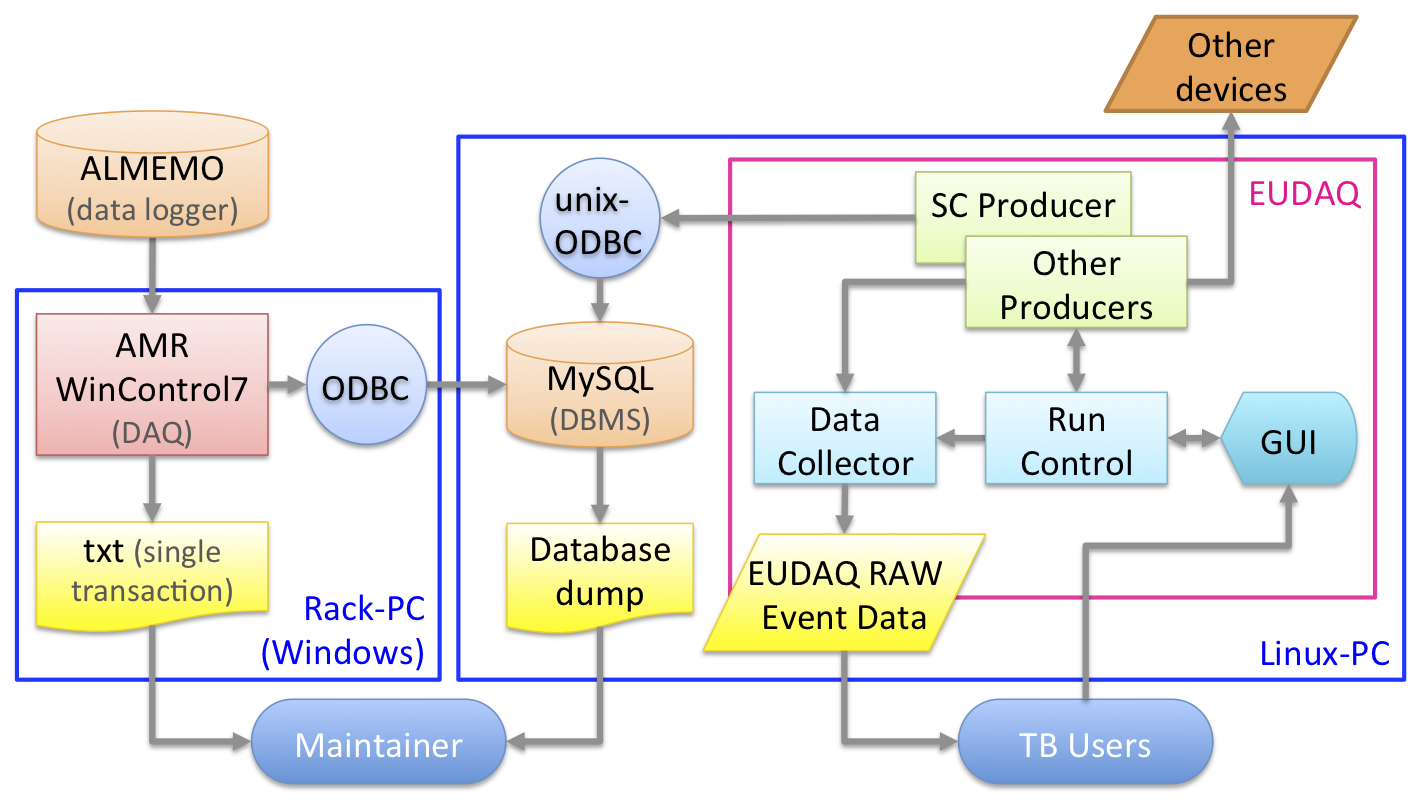
\includegraphics[trim={5cm .5cm 2cm 5cm},clip,width=\textwidth]{FlowChartSCS.png}
\caption{Flow chart of the Slow Control System}
\end{figure}

\section{Installation}
\subsection{MySQL}
The MySQL database on the Linux PC is the central interaction point of both DAQ softwares. First of all there has to be a user which can be used from multiple hostes. This is required so that the AMR software on the Windows PC can remotly access the database. Therefore the certain user has to get access privileges from different computers. Use the following command to open MySQL in you terminal: \\
\colorbox{lightgray}{\texttt{mysql -u username -p}} \\
Check if the user your are logged in with has rights to access from multiple hosts: \\
\colorbox{lightgray}{\texttt{mysql> SELECT user, host FROM mysql.user;}}\\
If there is no \% behind the username (Fig. 4) you are using, either use a different user with remote access or create a new user with this access: \\
\colorbox{lightgray}{\texttt{mysql> GRANT ALL PRIVILEGES ON *.* TO 'USERNAME'@'\%' IDENTIFIED BY 'PASSWORD';}}\\
Afterwards logged in as this user you can start to create your own database and tables: \\
\colorbox{lightgray}{\texttt{mysql> CREATE DATABASE \textit{Databasename};}}\\
Then you can choose to work with this database and create own tables and structure them: \\
\colorbox{lightgray}{\texttt{mysql> create table `tablename`(`counter` int unsigned zerofill auto\_increment,}}\\
\colorbox{lightgray}{\texttt{`timer` datetime NOT NULL, `value` double);}}\\

\begin{figure} [H]
\centering
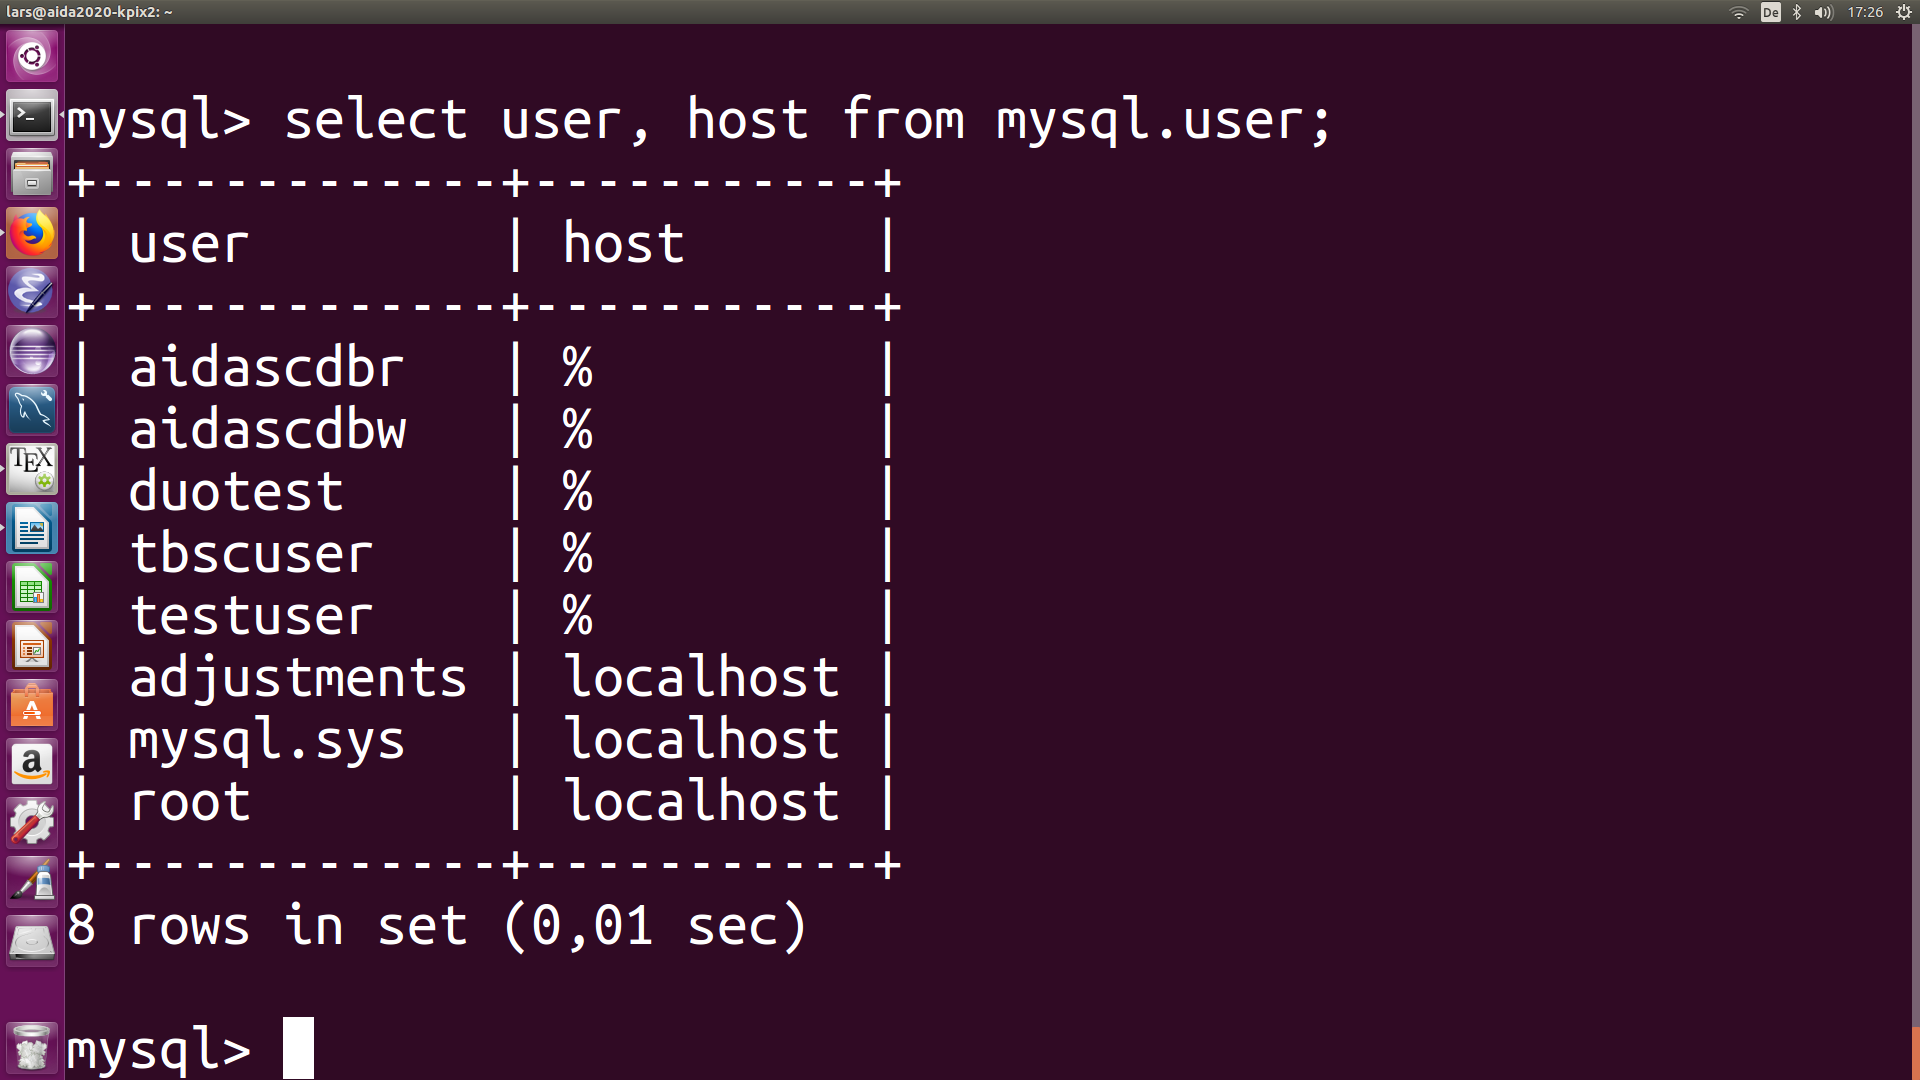
\includegraphics[trim={2cm 7cm 0cm 3cm},clip,width=\textwidth]{mysqluser.png}
\caption{check the access rights to hosts of your useraccount.}
\end{figure}

\subsection{ODBC}
The ODBC (Open DataBase Connectivity) is a general interface between different programms and databases. On the Windows PC has to be a ODBC/Connector for MySQL in a 32bit version [1] installed. \\
If this is installed a system DSN or user DSN can be created for a connection between the AMR software on the Windows PC and the MySQL database on the Linux PC. For creating a new DSN you have to open the ODBC data source administrator. \\ Click 'Add' under the register User or System DSN and continue with the configurations. \\
Name your new datasource and give the user with access rights to the MySQL database from multiple hosts. Choose the desired database for the transfared slow control data. For testing if your connection is working simply click on the 'Test' button.

\begin{figure} [H]
\centering
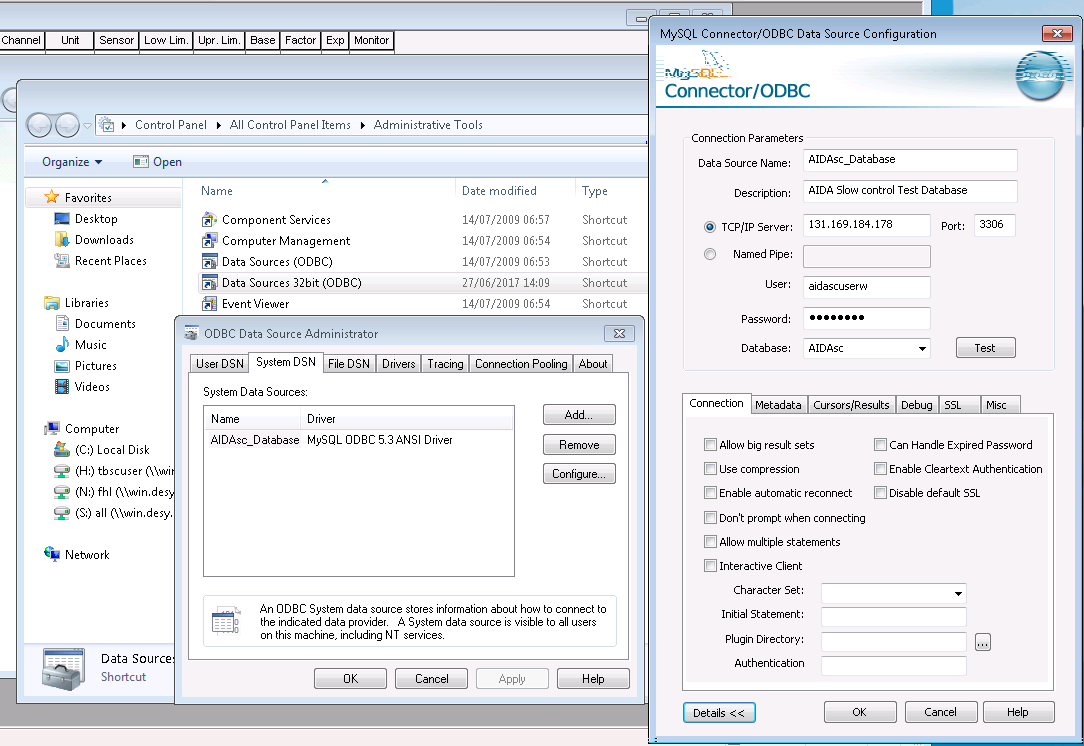
\includegraphics[width=\textwidth]{ODBC.png}
\caption{Adjust the properties of your ODBC DSN.}
\end{figure}

\subsection{unixODBC}
Thereby the EUDAQ framework can collect data from the MySQL database a unixDOBC has to be set up. It connects the different macros run by the EUDAQ RunControl with the MySQL database. There are two ways to create a new unixODBC connection. Before, please add this line to your shell setup (.bashrc): \\
\colorbox{lightgray}{\texttt{export ODBCSYSINI=/usr/local/etc}} \\ The first way is to change the odbcinst.ini file in the /etc directory of the Linux PC. A system DSN can just be added by the administrator or maintainer. \\
The second option to set up a unixODBC is to create a template file (Fig. 6) and add it to the DSNs of the PC. Specify the database, username and password, server and name the unixODBC in the squared brackets [2]. It is not of importance where the template file is stored. \\
To add the new unixODBC connection you only have to give the following command in the terminal [3]: \\
\colorbox{lightgray}{\texttt{odbcinst -i -s -f TemplateFileName}}\\
You can easy check if the ODBC has been added by showing all DSNs:\\
\colorbox{lightgray}{\texttt{odbcinst -q -s}}\\


\begin{figure} [H]
\centering
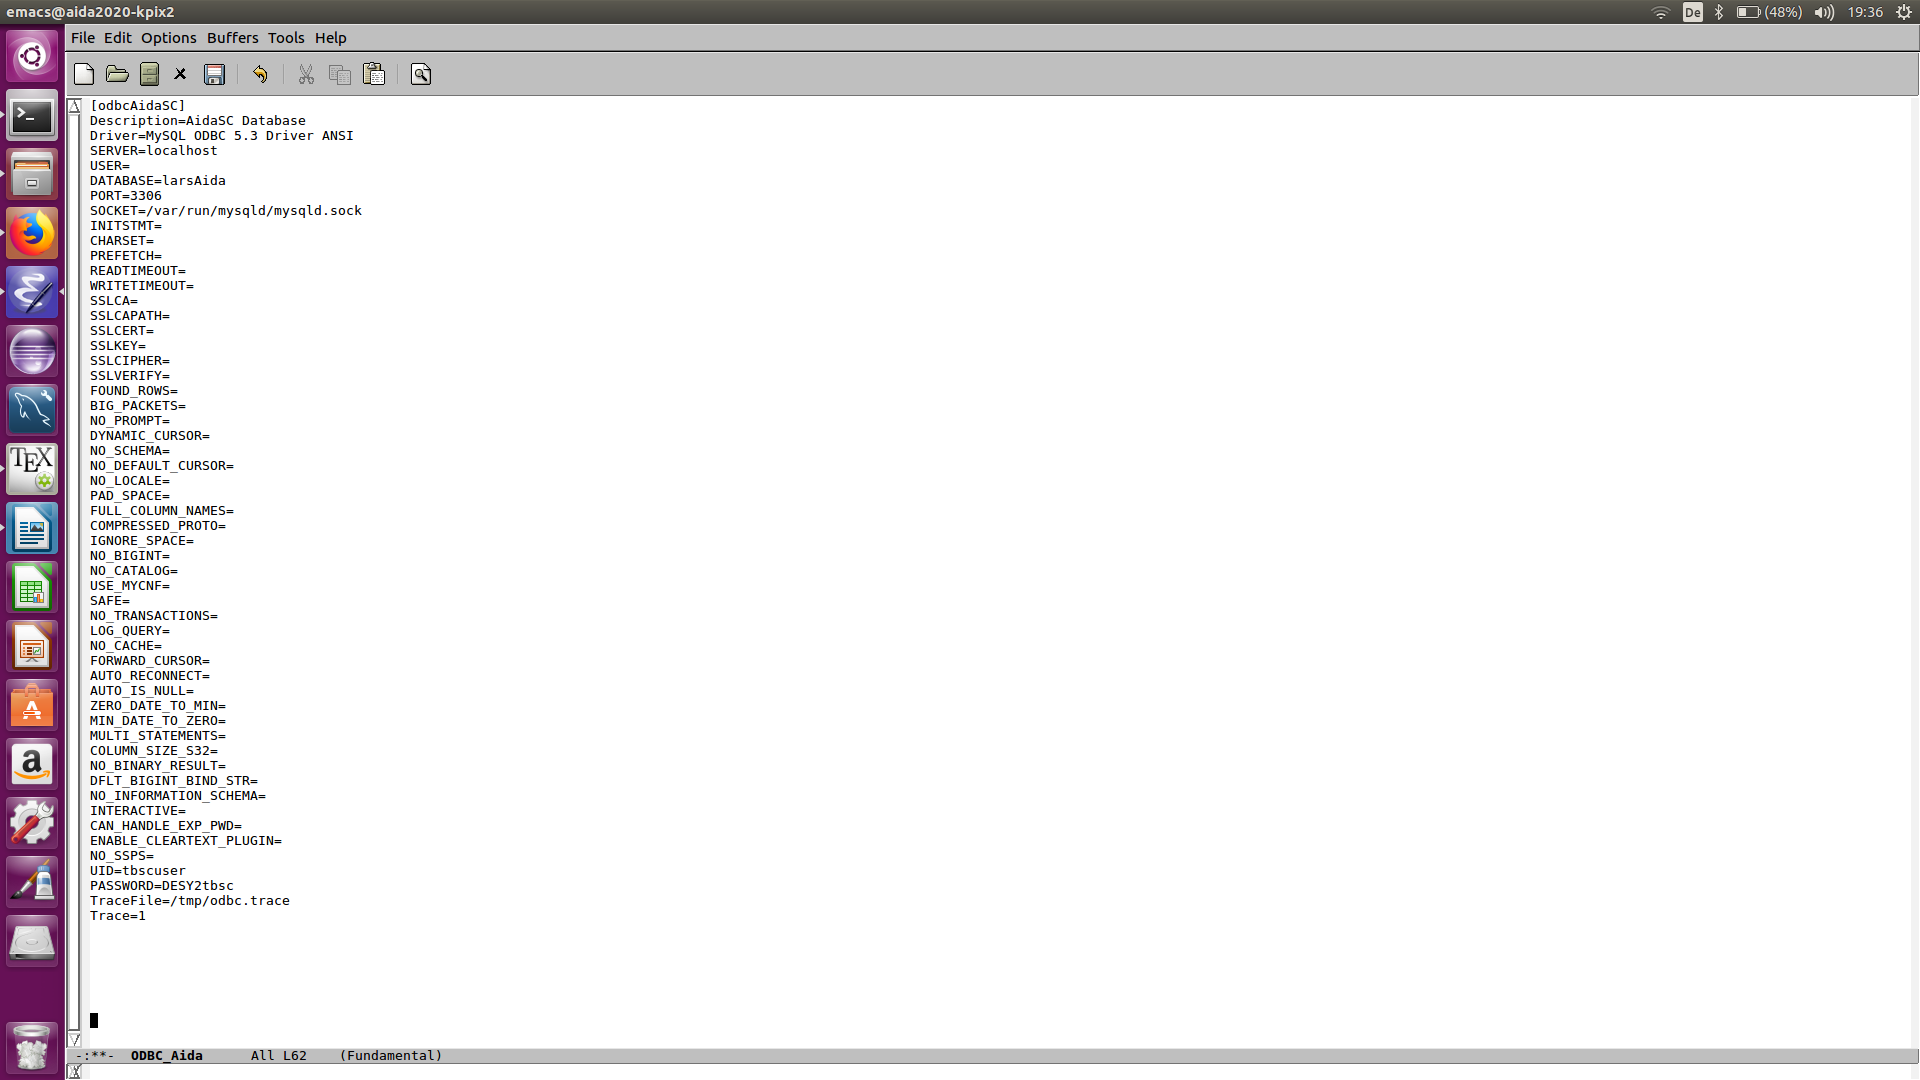
\includegraphics[trim={2.5cm 5cm 50cm 3.5cm},clip,width=7cm]{unixtemplate.png}
\caption{An example of a unixODBC template file.}
\end{figure}

\subsection{EUDAQ}
The EUDAQ framework was originally developed for the management of the Mimosa telescops (at DESY Duranta, Datura and Lycoris). The Slow Control System at DESY also uses the EUDAQ software to make it easyier to include to environmental parameters in other experimental datastreams. \\
The EUDAQ version used for the Slow Control System at DESY is stored and accessable in github [4]. To install this EUDAQ branch you follow the subsequent steps: \\
EUDAQ creates its own directory, you only have to run the command to install all files from the corresponding github repository: \\
\colorbox{lightgray}{\texttt{git clone https://github.com/MengqingWu/eudaq.git}} \\
After doing so you fetch the origin and check if the branch of your EUDAQ folder is mewu.master: \\
\colorbox{lightgray}{\texttt{git fetch origin}} \\
Check branch: \colorbox{lightgray}{\texttt{git branch}} \\
If the branch is not mewu.master, check into the right branch using: \\
\colorbox{lightgray}{\texttt{git checkout -b master orgin/mewu.master
}} \\
Befor continuing with the installtion make sure to have cmake or cmake-gui installed. You can do so by using:\\
\colorbox{lightgray}{\texttt{sudo apt-get install cmake}} or \colorbox{lightgray}{\texttt{sudo apt install cmake-qt-gui}}\\
Next of is the compilation with the makefiles. Create a /build directory under eudaq: \\
\colorbox{lightgray}{\texttt{mkdir build}} \\
And use the following command in this directory: \\
\colorbox{lightgray}{\texttt{cmake ..}} \\
Afterwards to finish the installation you use \\
\colorbox{lightgray}{\texttt{make install -j 4}}. \\

\section{Take Data}
When data taking there can occur multiple problems. The most common ones will be due to wrong connections in the conf file or because the AMR software is not polling. To illustrate the procedure of using the Slow Control System correctly there will be a short example:

\subsection{Operate the AMR software}
Open the AMR software in a remote Desktop via Ubuntu terminal(Fig. 7). \\
\colorbox{lightgray}{\texttt{xfreerdp /w:1600 /h:1000 /u:tbscuser /v:fhl-tb-sc01 /cert-ignore}} \\
make sure the ODBC connection is active, then click the red arrow in the top left corner. It should start blinking red and yellow when data is taken.

\begin{figure} [H]
\centering
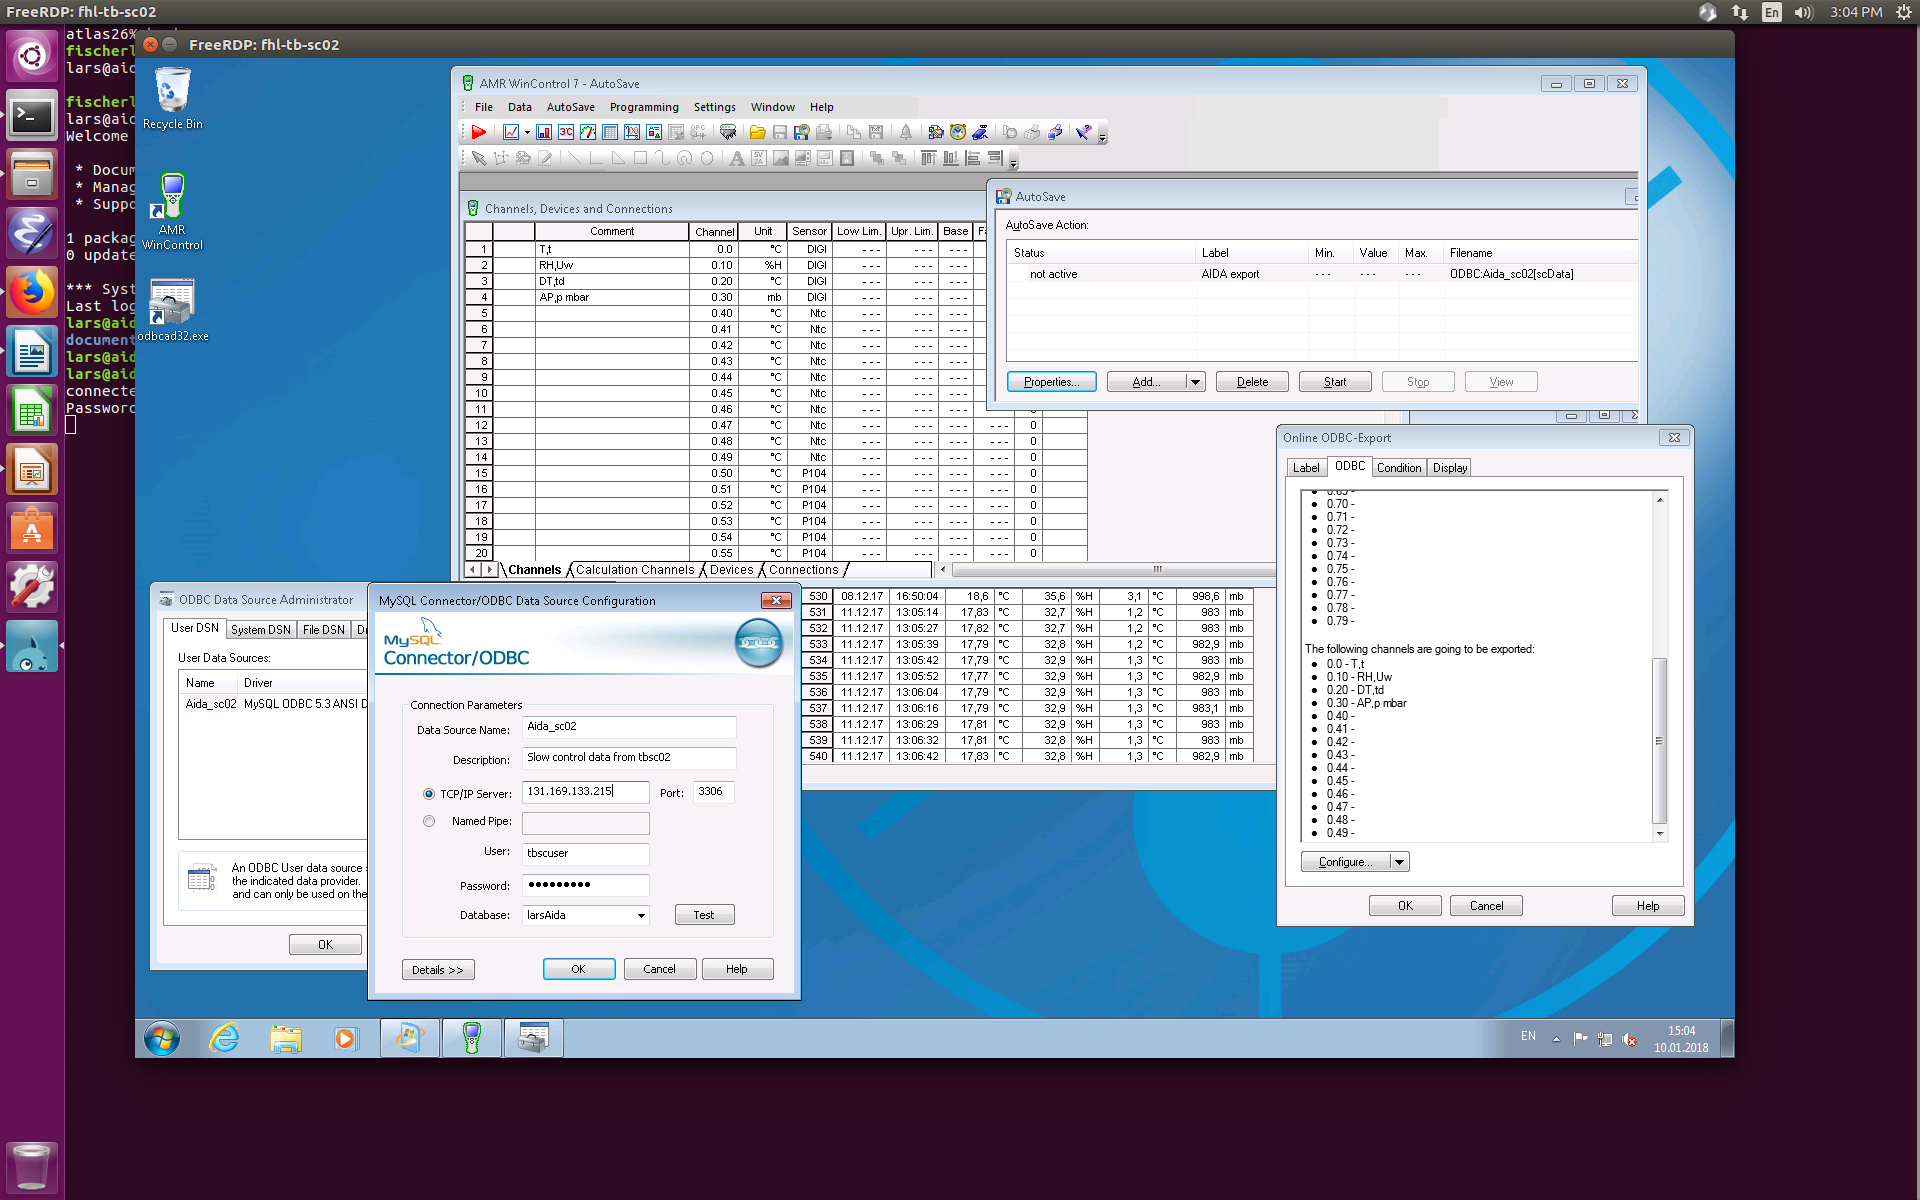
\includegraphics[trim={5cm 5cm 7cm 2cm},clip,width=\textwidth]{AMRSoftware.png}
\caption{AMR software (background) and ODBC connection (bottom left corner)}
\end{figure}

\subsection{Start EUDAQ}
To start EUDAQ go to the directory /bin and begin with running the GUI for the RunControl.\\
\colorbox{lightgray}{\texttt{./myeuRun}} \\
Use the Commands \\
\colorbox{lightgray}{\texttt{./euCliProducer -n tbscProducer -t tbsc}} \\
\colorbox{lightgray}{\texttt{./euCliCollector -n tbscDataCollector -t tbscDC}} \\
to start the Producer moduels and the DataCollector. All operations will be listed in the GUI of the RunControl.


\pagebreak
\section{References}
1: https://dev.mysql.com/downloads/connector/odbc/ \\
2: http://www.unixodbc.org/odbcinst.html \\
3: https://manpages.ubuntu.com/manpages/xenial/man1/odbcinst.1.html \\
4: https://github.com/MengqingWu/eudaq \\


\end{document}
